\documentclass [14 pt]{article}
\usepackage[a4paper, total={6in, 8in}]{geometry}

\usepackage{fancyhdr}

\usepackage{hyperref}
\usepackage{graphicx}
\usepackage{float}
\usepackage{color}
\usepackage[english]{babel}
\usepackage[utf8]{inputenc}
\usepackage{listings}
\usepackage{multicol}
\usepackage{subcaption}
\usepackage{multirow}
\usepackage{titling}
\renewcommand\maketitlehooka{\vfill}
\renewcommand\maketitlehookd{\vfill\null}

\definecolor{deepblue}{rgb}{0,0,0.5}
\definecolor{deepred}{rgb}{0.6,0,0}
\definecolor{deepgreen}{rgb}{0,0.5,0}

\lstset{
language=Python,
	belowcaptionskip=1\baselineskip,
  	frame=single,
  	numbers=left,
  	xleftmargin=\parindent,
  	basicstyle=\ttfamily\scriptsize,
  	showspaces=false,
  	showtabs=false,
 	breaklines=true,
  	showstringspaces=false,
  	breakatwhitespace=false,
    keywordstyle=\color{deepblue},
    stringstyle=\color{deepgreen},
    rulecolor= \color{black},
}

\linespread{1.25}

\title{Project 1: \href{https://github.com/SusyPinkBash/bad_smell_detection}{Bad Smell Detection}}
\author{Ardig\`o Susanna}
\begin{document}

\pagestyle{fancy}
\fancyhf{}
\lhead{Ardig\`o Susanna}
\rhead{Knowledge Analysis \& Management}
\cfoot{\thepage}

\begin{titlingpage}
\maketitle
\end{titlingpage}

\newpage\thispagestyle{plain}
\tableofcontents
\newpage

\section{Ontology Creation} % 1: intro
\subsection{Goal and Input parameter}
This part of the project consists of creating an ontology for Java Entities.\\
This file takes an optional argument which is the path of the python file that defines the Java Abstract Syntax Tree. If the argument is non supplied then a predefined path is used. For this project I used the file \texttt{tree.py} of the \href{https://github.com/c2nes/javalang}{Javalang} Python Library. 

\subsection{Parsing Classes}
In order to efficiently parse this file I created a class named \texttt{Class} to store the name, superclass and property of each class.
The function \texttt{get\_classes(python\_file\_name)} reads the given file, parses into an Abstract Syntax Tree. I use the function \texttt{walk} to iterate the tree, create instances of \texttt{Class} with the class definition nodes and save them into an array.\\
The main function \texttt{start} creates an ontology using the library \href{https://pythonhosted.org/Owlready2/}{Owlready2}. I then iterate the list of the parsed classes, previously explained, to create create in in the ontology. This step needs to differentiate among three different contruction creations depending on the number of superclasses.
If the current class has none, meaning that it has no super class, it is created as a subclass of Thing which, in owl, is the top superclass.
If the current class has one superclass, it is created as its subclass.
If the current class has two superclass, it is created as subclass of both.\\
For each class I add the previously extracted properties and add them to the ontology. There are two different types: 
Object, which are only \texttt{body} and \texttt{parameters}, and Data, which are all other properties.
Since the first type has only two possible values, I decided to add them only once at the end. To avoid conflict, when I create "name" properties I rename them to "jname".\\
The ontology is finally created and I can export it into an owl file.

\subsection{Results}
%TODO 1: results
\begin{figure}[H]
\centering
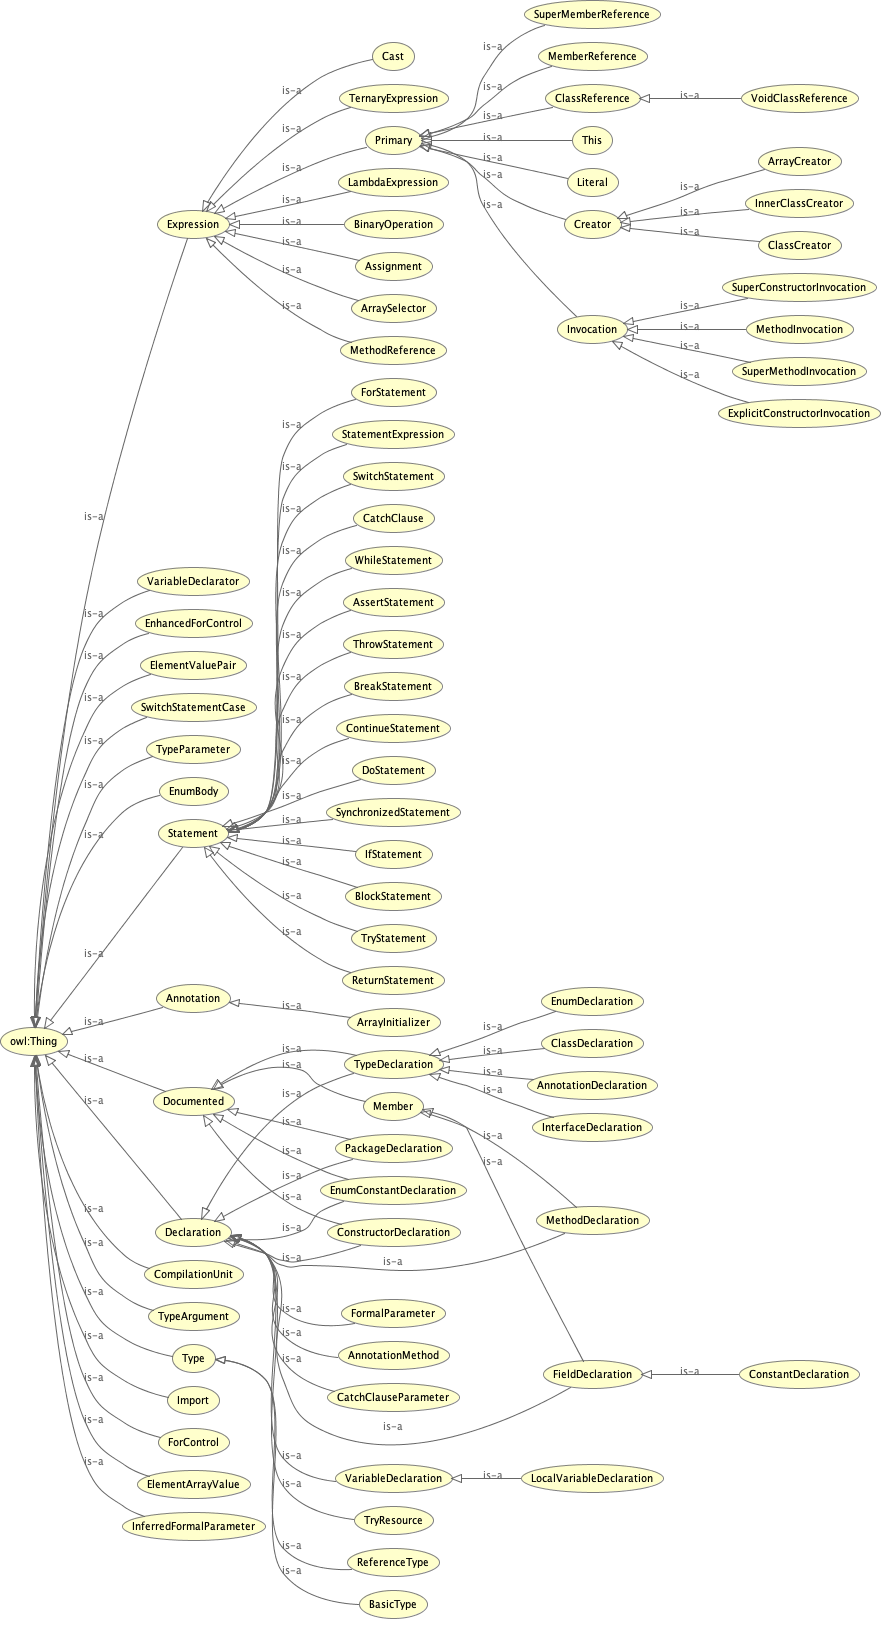
\includegraphics[height=0.9\textheight]{res/ontology_graph.png}
\caption{Class Hierarchy of the Ontology created}\label{fig:OntoClassGraph}
\end{figure}


\section{Populate the Ontology}
%Part 1: classes and class members
%Part 2: statements, method parameters

\subsection{Results}
%Table \ref{tab:TableFeatureVectors} shows the statistics computed in this section for each class. Each feature vectors represent a method of the class. Each entry in the vector refers to a method or field that is called or accessed at least once in that class.
%\begin{table}[H]
%\centering
%\begin{tabular}{l | c | c}
%\textbf{Class} &  \textbf{Number of Feature Vectors}	& \textbf{Length of the Feature Vectors}\\\hline
% CoreDocumentImpl	&	117 & 66 \\\hline
%   DTDGrammar		&	91 & 108 \\\hline
% XIncludeHandler	&	108 & 178 \\\hline
%  XSDHandler		&	106 & 193 \\
%\end{tabular}
%\captionof{table}{Feature vectors of each class found by \texttt{extract-feature-vectors.py}}\label{tab:TableFeatureVectors}
%\end{table}

\section{Find Bad Smell}

%\subsection{Clustering Algorithms}
%In this section I will use both K-Means and Hierarchical Agglomerative Algorithm to cluster the god classes. The algorithms are the only difference.\\ 
%These files take as input the path of the clustering csv and, as an optional argument, a value k.
%I create a Pandas Dataframe with the data of the given file, get the names of the methods and the value as a matrix (array of arrays).\\
%If the parameter k is given I only compute the values of such number for the given algorithm and export the clustering values to a csv. If k is not given I compute the values of all the possible k from 2 (it would be useful to have only one cluster) to a max k which I set to 60. At each step I save the values, using the Pandas describe, to then plot them on a graph.
%
%\subsubsection{K-Means}
%I used \href{https://scikit-learn.org/stable/modules/generated/sklearn.cluster.KMeans.html}{KMeans} from the library Scikit-learn with the following settings:
%\begin{itemize}
%	\item \texttt{n\_clusters = k} : number of clusters.
%	\item \texttt{init = k-means++} : the centroids initialisation.  
%	\item \texttt{n\_init = 10} : number of times the algorithm is run with different centroids.
%	\item \texttt{max\_iterint = 300} number of maximum iterations.
%	\item \texttt{algorithm = auto} : algorithm to use. In this case auto probably used \texttt{full} since the matrix is sparse.
%\end{itemize}
%I used the Euclidean Distance as a distance function.
%
%
%\subsubsection{Hierarchical Agglomerative} I
% used \href{https://scikit-learn.org/stable/modules/generated/sklearn.cluster.AgglomerativeClustering.html}{AgglomerativeClustering} from the library Scikit-learn with the following settings:
%\begin{itemize}
%	\item \texttt{n\_clusters = k} : number of clusters.
%	\item \texttt{linkage = ward} : this linkage rule is used to minimise the variance of the clusters merged.
%\end{itemize}

\subsection{Results}
%The goal is to analyze the informations of the different clustering results with different numbers of clusters computed by the two algorithms.
%Each plot shows the values of the minimum, mean, maximum and standard deviation (on the y axis) for each k in range 2 to 60 (on the x axis). The values decrease as the number of clusters increases. This is caused by the cluster sizes being bigger with small numbers of clusters k. \\\\
%Statistics of the class \texttt{CoreDocumentImpl} are shown in figure \ref{fig:CoreDocumentImpl0}.
%\begin{figure}[H]
%\centering
%\subcaptionbox{K-Means}{
% \includegraphics[width=0.45\textwidth]{../graphs/kmeans-CoreDocumentImpl.png}}
% \subcaptionbox{Hierarchical Agglomerative}{
%\includegraphics[width=0.45\textwidth]{../graphs/hierarchical-CoreDocumentImpl.png}}
%	\caption{Class CoreDocumentImpl: Statistics of cluster sizes}\label{fig:CoreDocumentImpl0}
%\end{figure}
%\noindent
%Statistics of the class \texttt{DTDGrammar} are shown in figure \ref{fig:DTDGrammar0}.
%\begin{figure}[H]
%\centering
%\subcaptionbox{K-Means}{
% \includegraphics[width=0.45\textwidth]{../graphs/kmeans-DTDGrammar.png}}
% \subcaptionbox{Hierarchical Agglomerative}{
%\includegraphics[width=0.45\textwidth]{../graphs/hierarchical-DTDGrammar.png}}
%	\caption{Class DTDGrammar: Statistics of cluster sizes}\label{fig:DTDGrammar0}
%\end{figure}
%\noindent
%Statistics of the class \texttt{XIncludeHandler} are shown in figure \ref{fig:XIncludeHandler0}.
%\begin{figure}[H]
%\centering\subcaptionbox{K-Means}{
%\includegraphics[width=0.45\textwidth]{../graphs/kmeans-XIncludeHandler.png}}
%\subcaptionbox{Hierarchical Agglomerative}{
%\includegraphics[width=0.45\textwidth]{../graphs/hierarchical-XIncludeHandler.png}}
%	\caption{XIncludeHandler: Statistics of cluster sizes}\label{fig:XIncludeHandler0}
%\end{figure}
%\noindent
%Statistics of the class \texttt{XSDHandler} are shown in figure \ref{fig:XSDHandler0}.
%\begin{figure}[H]
%\centering\subcaptionbox{K-Means}{
%\includegraphics[width=0.45\textwidth]{../graphs/kmeans-XSDHandler.png}}
%\subcaptionbox{Hierarchical Agglomerative}{
%\includegraphics[width=0.45\textwidth]{../graphs/hierarchical-XSDHandler.png}}
%	\caption{XSDHandler: Statistics of cluster sizes}\label{fig:XSDHandler0}
%\end{figure}

%
%Results of the class \texttt{XIncludeHandler} are shown in figure \ref{fig:XIncludeHandler}.
%\begin{figure}[H]
%\centering
%\includegraphics[width=0.4\textwidth]{../graphs/kmeans-XIncludeHandler.png}
%\includegraphics[width=0.4\textwidth]{../graphs/hierarchical-XIncludeHandler.png}
%	\caption{XIncludeHandler: K-Means (left) Hierarchical (right)}\label{fig:XIncludeHandler}
%\end{figure}
%
%Results of the class \texttt{XSDHandler} are shown in figure \ref{fig:XSDHandler}.
%\begin{figure}[H]
%\centering
%\includegraphics[width=0.4\textwidth]{../graphs/kmeans-XSDHandler.png}
%\includegraphics[width=0.4\textwidth]{../graphs/hierarchical-XSDHandler.png}
%	\caption{XSDHandler: K-Means (left) Hierarchical (right)}\label{fig:XSDHandler}
%\end{figure}

%\subsection{Silhouette}
%In this part I used \href{https://scikit-learn.org/stable/modules/generated/sklearn.metrics.silhouette_score.html}{silhouette\_score} from the library Scikit-learn.\\
%This file take as input the path of the feature vector and, as an optional argument, a file with the clustering.
%I create a Pandas Dataframe with the data of feature vectors, get the names of the methods and the value as a matrix (array of arrays).\\
%If the clustering is given I only compute the silhouette score of such cluster and print the result.
%If the cluster is not given I compute the values of all the possible k from 2 (it would be useful to have only one cluster) to a max k which I set to 60 of both k-means and hierarchical agglomerative algorithms. At each step I save the values of the scores into a Pandas Dataframe, to then plot them on a graph.
%I then look for the best score of both algorithms to give as output.
%
%
%\subsubsection{Results}
%The goal is to analyze the visualise the the different clustering results with different numbers of clusters computed by the two algorithms.
%Each plot shows the values of the silhouette score (on the y axis) for each k in range 2 to 60 (on the x axis). In two cases the values are initially high, they drop very fast to then slowly increase as the number of clusters increases. 
%\noindent
%This is caused by the cluster sizes being bigger with small numbers of clusters k. \\\\
%\noindent %class 1
%The class \texttt{CoreDocumentImpl} scored the highest value $0.7375460959$ with the Hierarchical algorithm at k equals to 43. The highest score of K-Means is $0.7350427350$ with k equals to 45. The plot of the results of this class is shown in figure \ref{fig:CoreDocumentImpl1}. In this graph we can see that, excluding the ends, both algorithms have similar score with the same k.
%For k greater than 45 the the score does not increase nor decrease. 
%
%\begin{figure}[H]
%\centering
%\includegraphics[width=0.65\textwidth]{../graphs/silhouette-CoreDocumentImpl.png}
%	\caption{CoreDocumentImpl: Silhouette metric}\label{fig:CoreDocumentImpl1}
%\end{figure}
%
%\noindent %class 2
%The class \texttt{DTDGrammar} scored the highest value $0.4369387011$ with the Hierarchical algorithm at k equals to 59. The highest score of K-Means is $0.4164393519$ with k equals to 59, as in the other algorithm. The plot of the results of this class is shown in figure \ref{fig:DTDGrammar1}. In this graph we can see that hierarchical has a higher score at most k and k-means has significantly low peaks at certain values.
% 
%\begin{figure}[H]
%\centering
%\includegraphics[width=0.65\textwidth]{../graphs/silhouette-DTDGrammar.png}
%	\caption{DTDGrammar: Silhouette metric}\label{fig:DTDGrammar1}
%\end{figure}
%
%\noindent %class 3
%The class \texttt{XIncludeHandler} scored the highest value $0.6708290353$ at k equals to 2 with the both algorithms. The plot of the results of this class is shown in figure \ref{fig:XIncludeHandler1}. The values of the first k are similar, then the hierarchical score tends to be more stable than the k-means which is has many peaks.
%
%\begin{figure}[H]
%\centering
%\includegraphics[width=0.65\textwidth]{../graphs/silhouette-XIncludeHandler.png}
%	\caption{XIncludeHandler: Silhouette metric}\label{fig:XIncludeHandler1}
%\end{figure}
%
%\noindent %class 2
%The class \texttt{XSDHandler} scored the highest value $0.5706530265$ with the K-Means algorithm at k equals to 2. The highest score of  Hierarchical is $0.5366896766$ with k equals to 2, as in the other algorithm. The plot of the results of this class is shown in figure \ref{fig:XSDHandler1}. The trend of the two algorithms is similar but the hierarchical is more stable while k-means, as in the previous cases, has more peaks. The highest scores are at with low values of k.
%
%\begin{figure}[H]
%\centering
%\includegraphics[width=0.65\textwidth]{../graphs/silhouette-XSDHandler.png}
%	\caption{XSDHandler: Silhouette metric}\label{fig:XSDHandler1}
%\end{figure}


%Results of the class \texttt{XSDHandler} are shown in figure \ref{fig:DTDGrammar1}.
%\begin{figure}[H]
%\centering
%\includegraphics[width=0.7\textwidth]{../graphs/silhouette-DTDGrammar.png}
%	\caption{DTDGrammar: Silhouette metric}\label{fig:DTDGrammar1}
%\end{figure}
%
%Results of the class \texttt{XSDHandler} are shown in figure \ref{fig:XIncludeHandler1}.
%\begin{figure}[H]
%\centering
%\includegraphics[width=0.7\textwidth]{../graphs/silhouette-XIncludeHandler.png}
%	\caption{XIncludeHandler: Silhouette metric}\label{fig:XIncludeHandler1}
%\end{figure}
%
%Results of the class \texttt{XSDHandler} are shown in figure \ref{fig:XSDHandler1}.
%\begin{figure}[H]
%\centering
%\includegraphics[width=0.7\textwidth]{../graphs/silhouette-CoreDocumentImpl.png}
%	\caption{CoreDocumentImpl: Silhouette metric}\label{fig:XSDHandler1}
%\end{figure}
%
%The best results of the two algorithms are:
%\begin{table}[H]
%\centering
%\begin{tabular}{l | c | c | c}
%\textbf{Class} & \textbf{Algorithm} & \textbf{k}	&\textbf{Score} \\\hline
% \multirow{2}{*}{CoreDocumentImpl} & K-Means & 45 & 0.7350427350427351 \\
% & Hierarchical &43 & 0.7375460958872944 \\\hline
% 
%  \multirow{2}{*}{DTDGrammar} & K-Means & 59 & 0.7350427350427351 \\
% & Hierarchical &59 & 0.7375460958872944 \\\hline
% 
%  \multirow{2}{*}{XIncludeHandler} & K-Means & 45 & 0.7350427350427351 \\
% & Hierarchical &43 & 0.7375460958872944 \\\hline
% 
%   \multirow{2}{*}{XSDHandler} & K-Means & 45 & 0.7350427350427351 \\
% & Hierarchical &43 & 0.7375460958872944 \\\hline
% 
%
%\end{tabular}
%\end{table}


%\section{Evaluation}
%In order to measure the quality of my solution I need to compare it with the real solution which I do not have. Thus I need to create a ground truth before computing the quality.
%
%
%\subsection{Ground Truth}
%I try to approximate a ground truth by dividing the methods into clusters based on a given keywords file. The file I used is:
%\lstinputlisting[language=Bash]{../keywords.txt}
%This python file takes as input the path to the feature vector csv and the keywords files.
%I create a list of the names of the methods importing the csv file into a Pandas frame to then retrieve the methods names.
%I create a list of the keywords, reading the text file, splitting on the new line character, casting it to set and the back to list to avoid doubles. At last I add \texttt{<none>} at the end of the list and check if there is any empty string. 
%In the next part I iterate through the methods, check if it contains any of the keyword to add it to the correct cluster. If it does not belong to any it is classified to the none.
%At last I create a Pandas Dataframe and export it to csv.
%
%\subsubsection{Results}
%Table \ref{tab:TableGroundTruth} shows the number of clusters, feature vectors and the size of the cluster \texttt{$<$none$>$} of each class. The last information is important because the higher the number in such cluster the less accurate our ground truth is. All classes have at least half of the data in this particular cluster.
%\begin{table}[H]
%\centering
%\begin{tabular}{l | c | c | c}
%\textbf{Class} & \textbf{Clusters}	&\textbf{Feature Vectors} & \textbf{Size of cluster $<$none$>$}\\\hline
% CoreDocumentImpl	&	11 & 	117 & 69 \\\hline
%   DTDGrammar		&	5 & 	91 	& 64 \\\hline
%    XIncludeHandler	&	6 & 	108 & 90 \\\hline
% XSDHandler			&	6 & 	106 & 57 \\
%\end{tabular}
%\captionof{table}{Statistics of Ground Truth for class found by \texttt{ground-truth.py}}\label{tab:TableGroundTruth}
%\end{table}
%
%\subsection{Precision and Recall}
%The precision is defined as:
%$$ p = \frac{\mid intrapairs (D[k]) \cap intrapairs (G) \mid}{\mid intrapairs (D[k])\mid}$$
%The recall is defined as:
%$$ r = \frac{\mid intrapairs (D[k]) \cap intrapairs (G) \mid}{\mid intrapairs (G)\mid}$$
%F1 is defined as:
%$$ F_1 = \frac{2\cdot p\cdot r}{p+r}$$
%\noindent
%The python file takes as input the clustering and ground truth path files.  The first file is the best among the computed among the different cluster sized and the two different algorithms based on the silhouette score. \\
% I create a Pandas Dataframe for both and compute the intrapairs (pairs of nodes of the same cluster). To compute them I groupby the cluster, iterate each group and, if it's not the same element, I add it to a set to avoid duplicates. With the pairs I have all the informations needed to compute this metrics.
%
%\subsubsection{Results}
%Table \ref{tab:TablePrecRecall} shows the results of precision, recall and F of each class.
%\begin{table}[H]
%\centering
%\begin{tabular}{l | c | c | c}
%\textbf{Class} & \textbf{Precision}	&\textbf{Recall} & \textbf{F}\\\hline
% CoreDocumentImpl	&	0.6757990868 & 	0.2965931864 & 0.4122562674 \\\hline
%   DTDGrammar		&	0.8561151079 & 	0.0548639926 & 	0.1031195841 \\\hline
% XIncludeHandler	&	0.6933919092 & 	0.9355396394 & 0.7964676198 \\\hline
% XSDHandler			&	0.3511731627 & 	0.8952051409 & 0.5044568245 \\
%\end{tabular}
%\captionof{table}{Statistics of each class found by \texttt{prec-recall.py}}\label{tab:TablePrecRecall}
%\end{table}
%
%\subsection{Discussion}
%I think that automating the clustering of god classes can be useful if the results are correct. In this case I did not have a real solution to check and I had to create my own ground truth. The results are probably not precise since the such ground truth was created with clustering based on some keywords that were matched with method names. 
%I think that this project is potentially very useful and powerful to find and fix potential problems in projects.
%
%\section{How to run the project}
%I created a bash script to run effortlessly the whole project.\\
%All the data and the graphs are saved into the folder with the same name.\\
%To automate the data processing the path of the god classes are saved into a file which is then read and given as input to extract the feature vectors. The clustering part executes  k-means, hierarchical and silhouette. This last file saves the best k and the algorithm to use which is then used to call the correct file with the correct parameter. For the evaluation I first calculate all the ground truth and then the precision and recall metrics.

\newpage
\appendix

\section{Python code}

\subsection{Project}
\subsubsection{Create Ontology}
\lstinputlisting{./src/onto_creator/onto_creator.py}
\subsubsection{Populate Ontology}
\lstinputlisting{./src/individ_creator/individ_creator.py}
\subsubsection{Find Bad Smell}
\lstinputlisting{./src/bad_smells/bad_smells.py}

\subsection{Tests}
\subsubsection{Create Ontology}
\lstinputlisting{./src/onto_creator/onto_creator_tests.py}
\subsubsection{Populate Ontology}
\lstinputlisting{./src/individ_creator/individ_creator_tests.py}
\subsubsection{Find Bad Smell}
\lstinputlisting{./src/bad_smells/bad_smells_tests.py}



\section{Bash Code} 
\subsection{Run Project}
\lstinputlisting[language=Bash]{./run.sh}
\subsection{Test Project}
\lstinputlisting[language=Bash]{./test.sh}


\end{document}